% Appendix A

\chapter{Navier-Stokes equation in Spectral Element Formulation } % Main appendix title

\label{AppendixA} % For referencing this appendix elsewhere, use \ref{AppendixA}

\lhead{Appendix A. \emph{NS Equations in SEM formuation}} % This is for the header on each page - perhaps a shortened title
\section{Weak Formulation of NS: Galerkin projection}\label{galproj}
   
${\Omega} \subset \mathbb{R}^{3}$ $\Rightarrow$ domain of NS equation. 
 Sobolev spaces for velocity and pressure $X:= H_0^{1}(\Omega)^3$ and $Z:= L_{0}^{2}(\Omega)$ respectively
\begin{eqnarray}
L_{0}^{2}(\Omega)  & = &   \left\{ q \in L^2(\Omega) \ \Bigg| \int_{\Omega}q d^{3}\pmb{x} = 0 \right\} \\ 
H^{1}(\Omega) & = & \left\{ q \in L^2(\Omega) \ \vert \alpha \vert \leq 1, \ \Bigg| D^{\alpha}q \in L^2(\Omega)  \right\} \\
H_0^{1}(\Omega)    & = & \left\{ q \in H^1(\Omega) \ \Bigg| q \Big \vert_{\partial \Omega} = 0 \right\} 
\end{eqnarray}
where $D^{\alpha} = {\partial ^{\alpha}}/{\partial x_1^{\alpha_1}\partial x_2^{\alpha_2}\partial x_3^{\alpha_3}}$, with $\vert \alpha \vert = \alpha_1 + \alpha_2 + \alpha_3$, is the distributional derivative operator.

The variational formula of the NS equation (used in Nek5000 implementation) can be derived by projecting the residual in an orthogonal test space, with test function $\pmb{v}\ \in \ H^{0}_{1}(\Omega)^{3}$.
\begin{equation}
\int_{\Omega} \pmb{v}\cdot \frac{\partial \pmb{u}}{\partial t}\mbox{d} \Omega +  \int_{\Omega} \pmb{v}\cdot \pmb{u} \cdot \nabla \pmb{u}\mbox{d} \Omega = -\int_{\Omega} \pmb{v}\cdot \nabla p\mbox{d} \Omega + \frac{1}{Re} \int_{\Omega} \pmb{v}\cdot \nabla ^{2} \pmb{u}\mbox{d} \Omega + \int_{\Omega} \pmb{v}\cdot \pmb{f}\mbox{d} \Omega
\end{equation}
or in a simplified way
\begin{equation}
\int_{\Omega}\mathfrak{{R}}(\pmb{u})\pmb{v}d^{3}\pmb{x} = 0 \ \ \ \ \ \forall\pmb{v}\in X, \label{res}
\end{equation}
where the residual $\mathfrak{{R}}$ in Equation(~\ref{res})
\begin{equation}
 \mathfrak{{R}}(\pmb{u}) = \frac{\partial \pmb{u}}{\partial t} + \pmb{u}.\nabla \pmb{u} + \frac{1}{\rho}\nabla p + \pmb{f} - \nu \nabla^2 \pmb{u}
\end{equation} 
 is orthogonally projected to the test space (same as trial space in Galerkin projection: we use the notation $( \ , \ )$ for complete integration for projection for brevity). Similar procedure is performed for the continuity equation,
\begin{equation}
\left(\frac{\partial{\pmb{u}}}{\partial t}, \pmb{v}\right) + \left(\pmb{u}\nabla \pmb{u},\pmb{v}\right) = -\left(\nabla p ,\pmb{v}\right) + \left(\pmb{f} , \pmb{v}\right) + \left(\nu \nabla^{2} \pmb{u}, \pmb{v}\right) \ \ \ \ \forall\pmb{v}\in X, \label{weak1}
\end{equation}

\begin{equation}
\left( q , \nabla.\pmb{u}\right) = 0 \ \ \ \ \ \ \forall {q}\in Z. \label{weak2}
\end{equation}


In discrete space, the trial and and test spaces for 3-dimensional velocity field is $X^N \subset X$ and scalar pressure field is $Z^N \subset Z$ where $X^{N}, Z^{N}$ are finite polynomial function subspaces with $N$ being the degree of the polynomial.\\
\par
If $E$ is the total number of non-overlapping elements in SEM, with the non-overlapping domains as $\cup_{e=1}^{E}\Omega_{e}$, the discrete subspaces for velocity and pressure can be represented as 
$X_N = X\cap \mathbb{P}_{N,E}^{3}$ and $Z_N = Z\cap \mathbb{P}_{N-2,E}^{3}$, where $\mathbb{P}_{N,E}$ can be given by
\begin{equation}
\mathbb{P}_{N,E} = \left\{ \psi \ \Big|\ \psi \in L^2(\Omega); \:\:\psi|_{\Omega_e} \mbox{Lagrange-Legendre polynomial of degree} \leq N \right\}. \label{sob2}
\end{equation}
and $\mathbb{P}_{N-2,E}$ can be given as
\begin{equation}
\mathbb{P}_{N-2,E} = \left\{ \phi \ \Big|\ \phi \in L^2(\Omega); \:\:\phi|_{\Omega_e} \mbox{Lagrange-Legendre polynomial of degree} \in \ (1, \ N-1) \right\}. \label{sob3}
\end{equation}

\section{Tensor Products: Derivatives}\label{tens}
The mapping of vector representation of the nodal coefficients $u_{ijk}^{e}$
\begin{equation}
\underline{u}^{e} = (u_{000}^e, u_{100}^e, \ldots , u_{ijk}^e, \ldots, u_{N_xN_yN_z}^e)^T=(u_1, u_2,\ldots, u_l, \ldots, u_{\mathcal{N}})^T 
\end{equation}
where $\mathcal{N} = (N_x+1)(N_y+1)(N_z+1)$ is the number of basis coefficients in a given element, and the mapping translates from three-index coefficient representation to a standard vector which is referred to as the natural or lexicographical ordering.
$\hat{D}_x$ the matrix operator for the one dimensional derivative in $x$ direction; $\hat{D}_x$ is of size $(N_x+1)\times (N_x+1)$ obtained from the values of derivative of Lagrange-Legendre interpolating polynomial associated with $N_x + 1$ GLL points on the reference interval $[-1, 1]$ applied to each $N_x+1$-dimensional vector $(u_{0jk}^e,u_{1jk}^e, \ldots, u_{N_xjk}^e)^T$, $j = 0, \ldots, N_y$, $k = 0, \ldots, N_z$. We define analogously $\hat{D}_y$, $\hat{D}_z$ for one dimensional derivatives in $y,z$ direction.

Kronecker product of two matrices $A$ of size $k\times l$ and $B$ of size $m\times n$ as the matrix $C = A\otimes B$ of size $km\times ln$ given as 
\begin{equation}
c_{ij} = a_{pq}b_{rs},  \ \ \  0\le i\le km,  0\le j\le ln,
\end{equation}
where the index pairs $pq$ and $rs$ satisfy the relationships
\begin{equation}
i = r + (p-1)m ,      j = s + (q-1)n.
\end{equation}

 Based on the lexicographical ordering of $\underline{u}$, the block diagonal matrix format of the derivatives in $x,y,$ and $z$ direction as Kronecker or tensor product form can be given as $D_x = I_y\otimes I_z\otimes \hat{D}_x$, $D_y = I_x\otimes \hat{D}_y\otimes I_z$ and $D_z = \hat{D}_z\otimes I_x\otimes I_y$, where $I_x$ is the identity matrix of size $(N_x+1)\times (N_x+1)$ and so on.


\section{Legendre polynomials}\label{legpol}

Legendre polynomials are finite series polynomial solutions to a special class of differential equations with parameter $n$.
\begin{equation}
(1-x^{2})\frac{d^{2}y}{dx^{2}} -2x\frac{dy}{dx} + n(n+1)y = 0
\end{equation}
The polynomials are denoted by $L_{N}(x)$. The polynomials are even or odd functions of $x$ depending on even or odd orders of $n$. A first few Legendre polynomials are 
\begin{align*}
L_{0}(x) & = 1 \\
L_{1}(x) & = x \\
L_{2}(x) & = \frac{1}{2}(3x^2 - 1) \\
L_{4}(x) & = \frac{1}{2}(5x^3 - 3x)
\end{align*}
with $L_k(\pm 1) = (-1)^k$ representing the bounds of the polynomial.\\
Some of the important recursion relations that can be used to find the Legendre polynomials of higher order are given as
\begin{align}
{x^2-1 \over n} {d \over dx} L_n(x) & = xL_n(x) - L_{n-1}(x) \\
(n+1) L_{n+1}(x) & = (2n+1) x L_n(x) - n L_{n-1}(x) \\
(2n+1) L_n(x) & = {d \over dx} \left[ L_{n+1}(x) - L_{n-1}(x) \right]
\end{align}

The orthogonality of Legendre polynomials over $L^{2}$ inner product space ($-1 \le x \le 1$) can be given as
\begin{equation}
\int_{-1}^{1} L_p(x) L_q(x)\,dx = {2 \over {2q + 1}} \delta_{pq}
\end{equation}
where $\delta_{pq}$ is the Kronecker delta function.
Similarly orthogonality of the derivatives and  some modification Legendre polynomial (See Appendix~\ref{lagintp}) can also be established in a straightforward manner.
\section{Lagrange Interpolants}\label{lagintp}
  Roots of Lagrange Legendre polynomial for the velocity interpolants
\begin{equation}
(1-\xi_j^{2})L'_{N}(\xi_j) = 0, \ \ \ \forall \xi_j \in [-1,1]. \label{GLL}
\end{equation}
 Equation~(\ref{GLL}) is solved using Newton-Raphson technique with initial condition of $\xi_j = \cos(j\pi/N), \ \ j = 0,\ldots, N,$ for obtaining a fast convergence. $L'_{N}$ is the first derivative of $N^{th}$ order Legendre polynomial and all the roots lie between $\pm 1$ with a clustering near -1 and 1. These nodes are commonly referred to as Gauss-Lobatto-Legendre (GLL) quadrature points, with the quadrature weights
 
 \begin{equation}
 \rho_j = \frac{2}{N(N+1)}\frac{1}{[L_N(\xi_j)]^2}, \ \ \ \ 0 \le j\le N, \ \ \ \forall \xi_j\in [-1,1]. \label{weights}
 \end{equation}
 The quadrature weights in Equation~(\ref{weights}) are computed as a function of $N^{th}$ order Legendre polynomials at GLL quadrature points. The discrete inner product in 3D thus reduces to
\begin{equation}
(f,g)_{N} = \sum_{i,j,k=0}^{N}\rho_{ijk}f_{ijk}g_{ijk}.\label{galerkin3}
\end{equation}
Here $(f_{ijk},g_{ijk})$ are defined on 3D GLL quadrature nodes on a reference cube and quadrature weights are $\rho_{ijk} = \rho_{i}\rho_{j}\rho_{k}$.\\
Along the same lines we can define the qudrature points of pressure interpolants as the roots of Legendre polynomial, referred to as Gauss-Legendre (GL) quadrature points.
\begin{equation}
L_{N-1}(\zeta_j) = 0, \ \ \ \forall \zeta_j \in [-1, 1], \ \ 1\le j\le N-1 \label{GL}
\end{equation}
where the roots $\zeta$ are solved using Newton-Raphson method. Consequently, the quadrature weights of GL nodes are given as 
\begin{equation}
\rho^{p}_j = \frac{2}{(1 - \zeta_j^{2})[L'_{N-1}(\zeta_j)]^{2}} \ \ \ \ 1 \le j\le N-1, \ \ \ \forall \zeta_j\in [-1,1]
\end{equation}
with the discrete 3D inner products for $(f,g)_{N,GL}$ being similar to Equation(~\ref{galerkin3}), but with summation from $1$ to $N-1$ using weights $\rho^{p}_{ijk} = \rho^{p}_{i}\rho^{p}_{j}\rho^{p}_{k}$.
\begin{figure}
\centering
        \begin{subfigure}[b]{0.75\textwidth}
                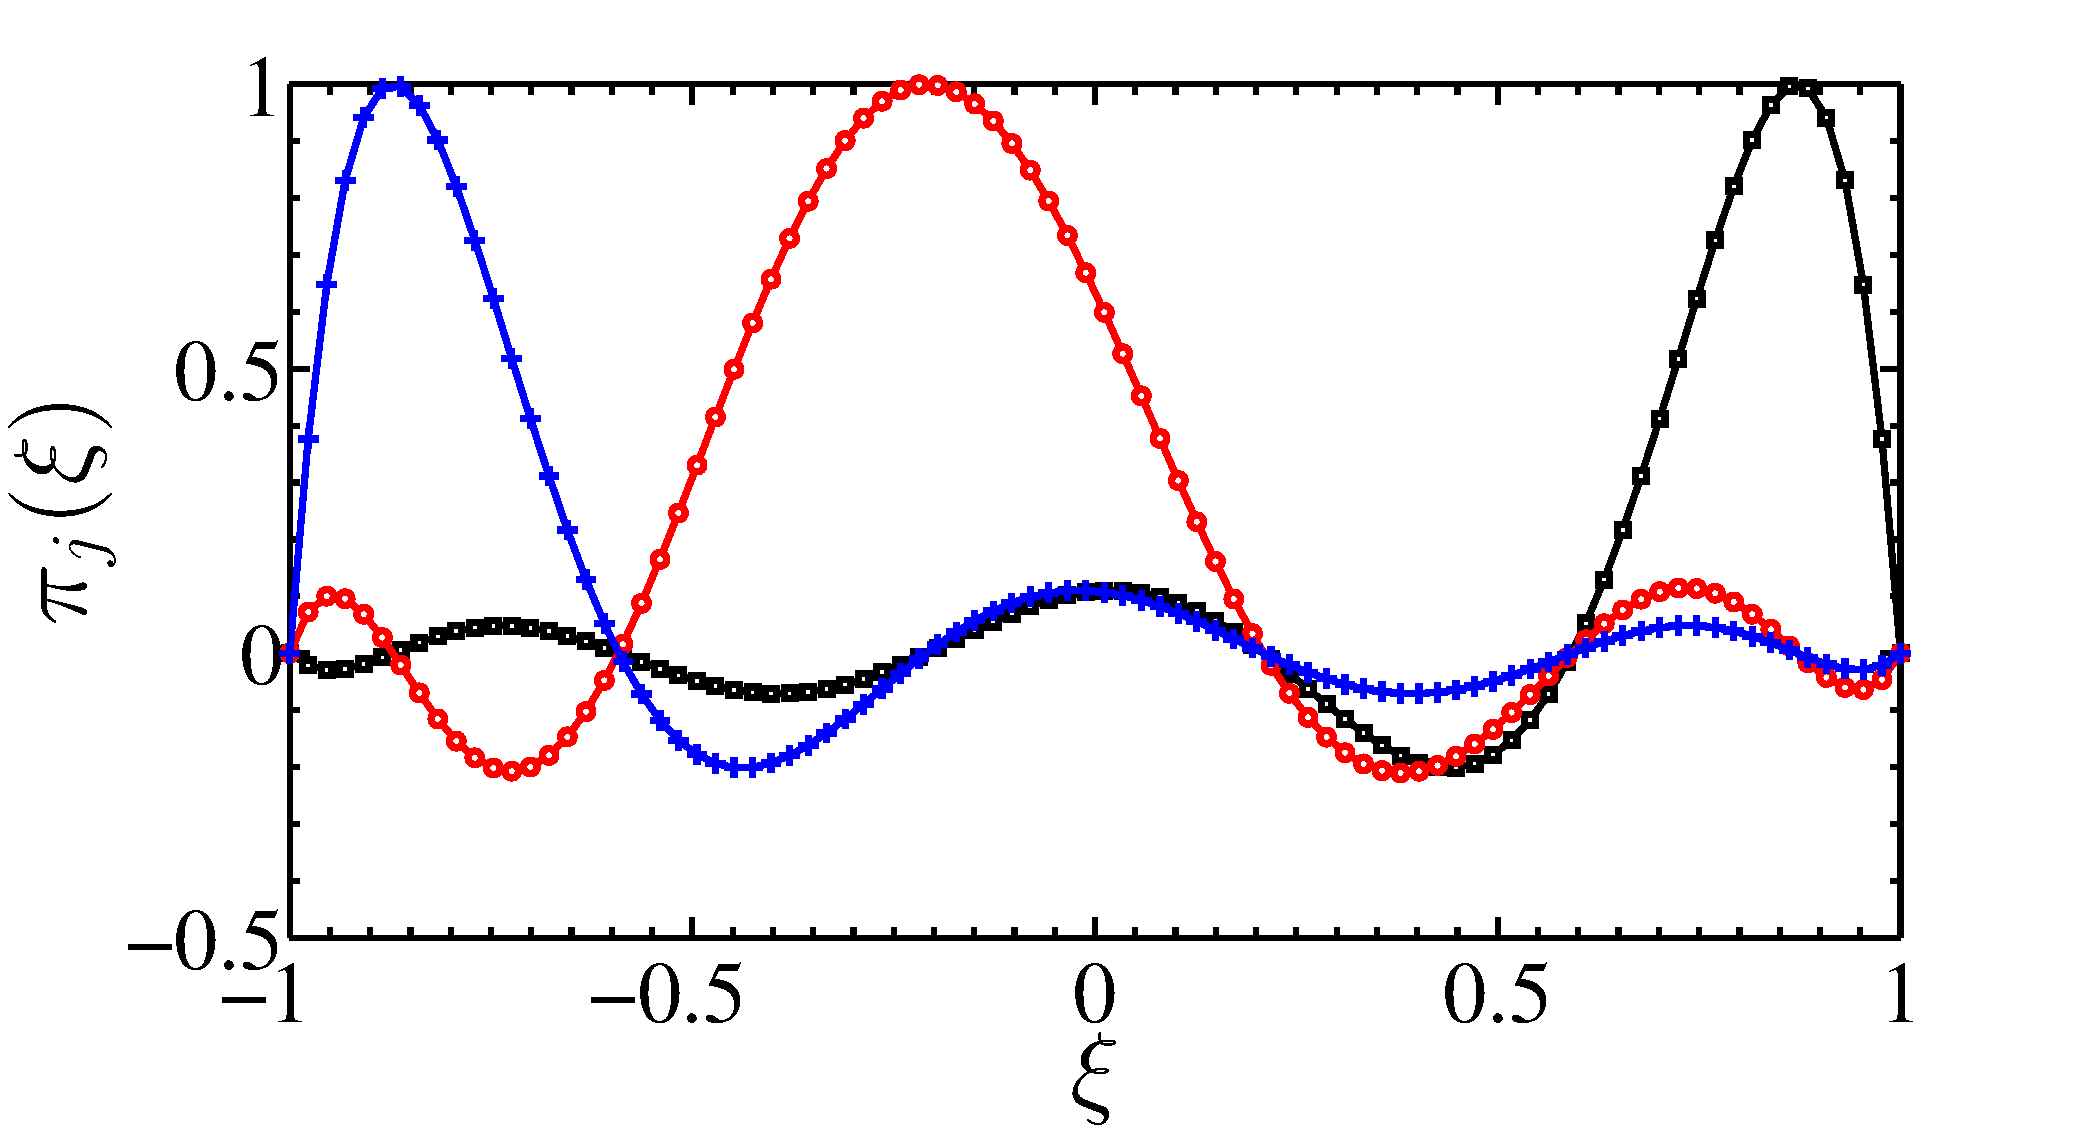
\includegraphics[width=\linewidth]{Figure/legpoly2.pdf}
                \caption{}
                \label{fig:poly1}
        \end{subfigure}
          \begin{subfigure}[b]{0.45\textwidth}
         \centering
                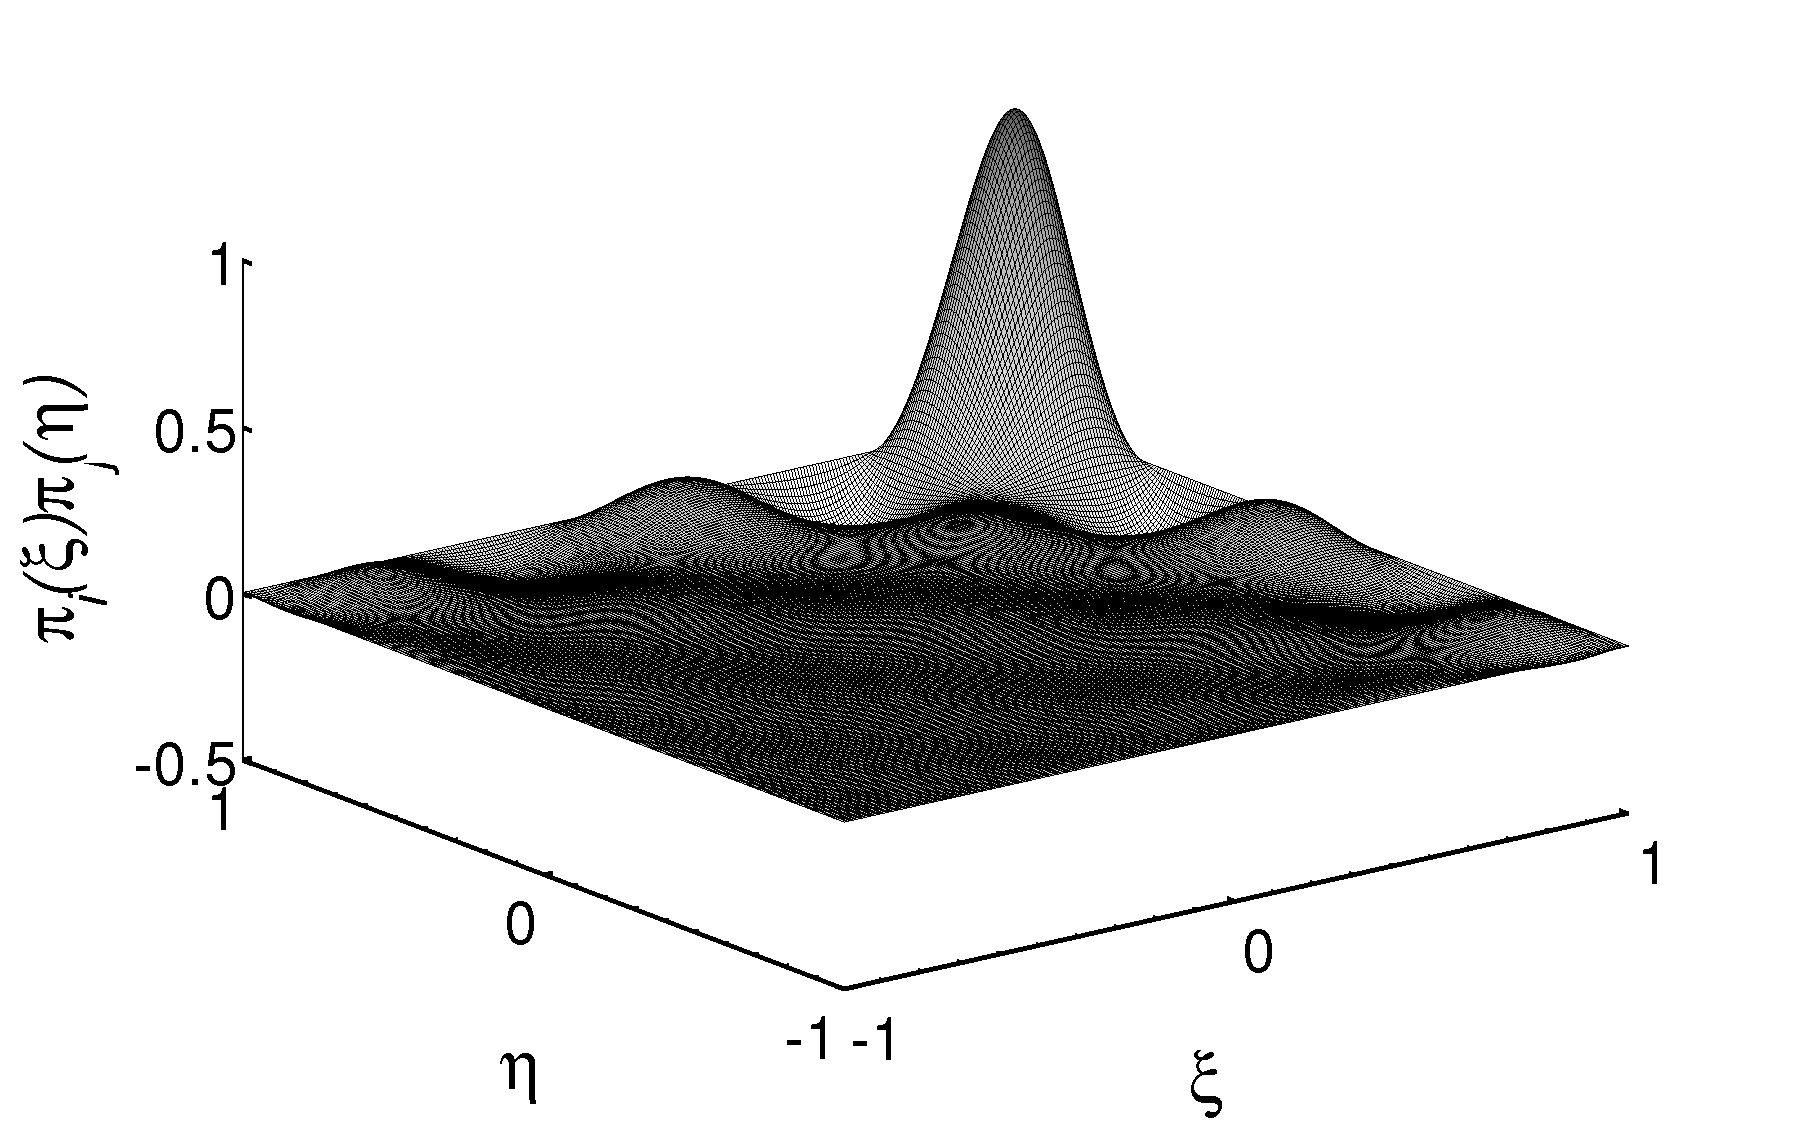
\includegraphics[width=\linewidth]{Figure/legpoly_2D1.pdf}
                 \caption{}
                 \label{fig:poly2}
         \end{subfigure}%
         \begin{subfigure}[b]{0.45\textwidth}
         \centering
                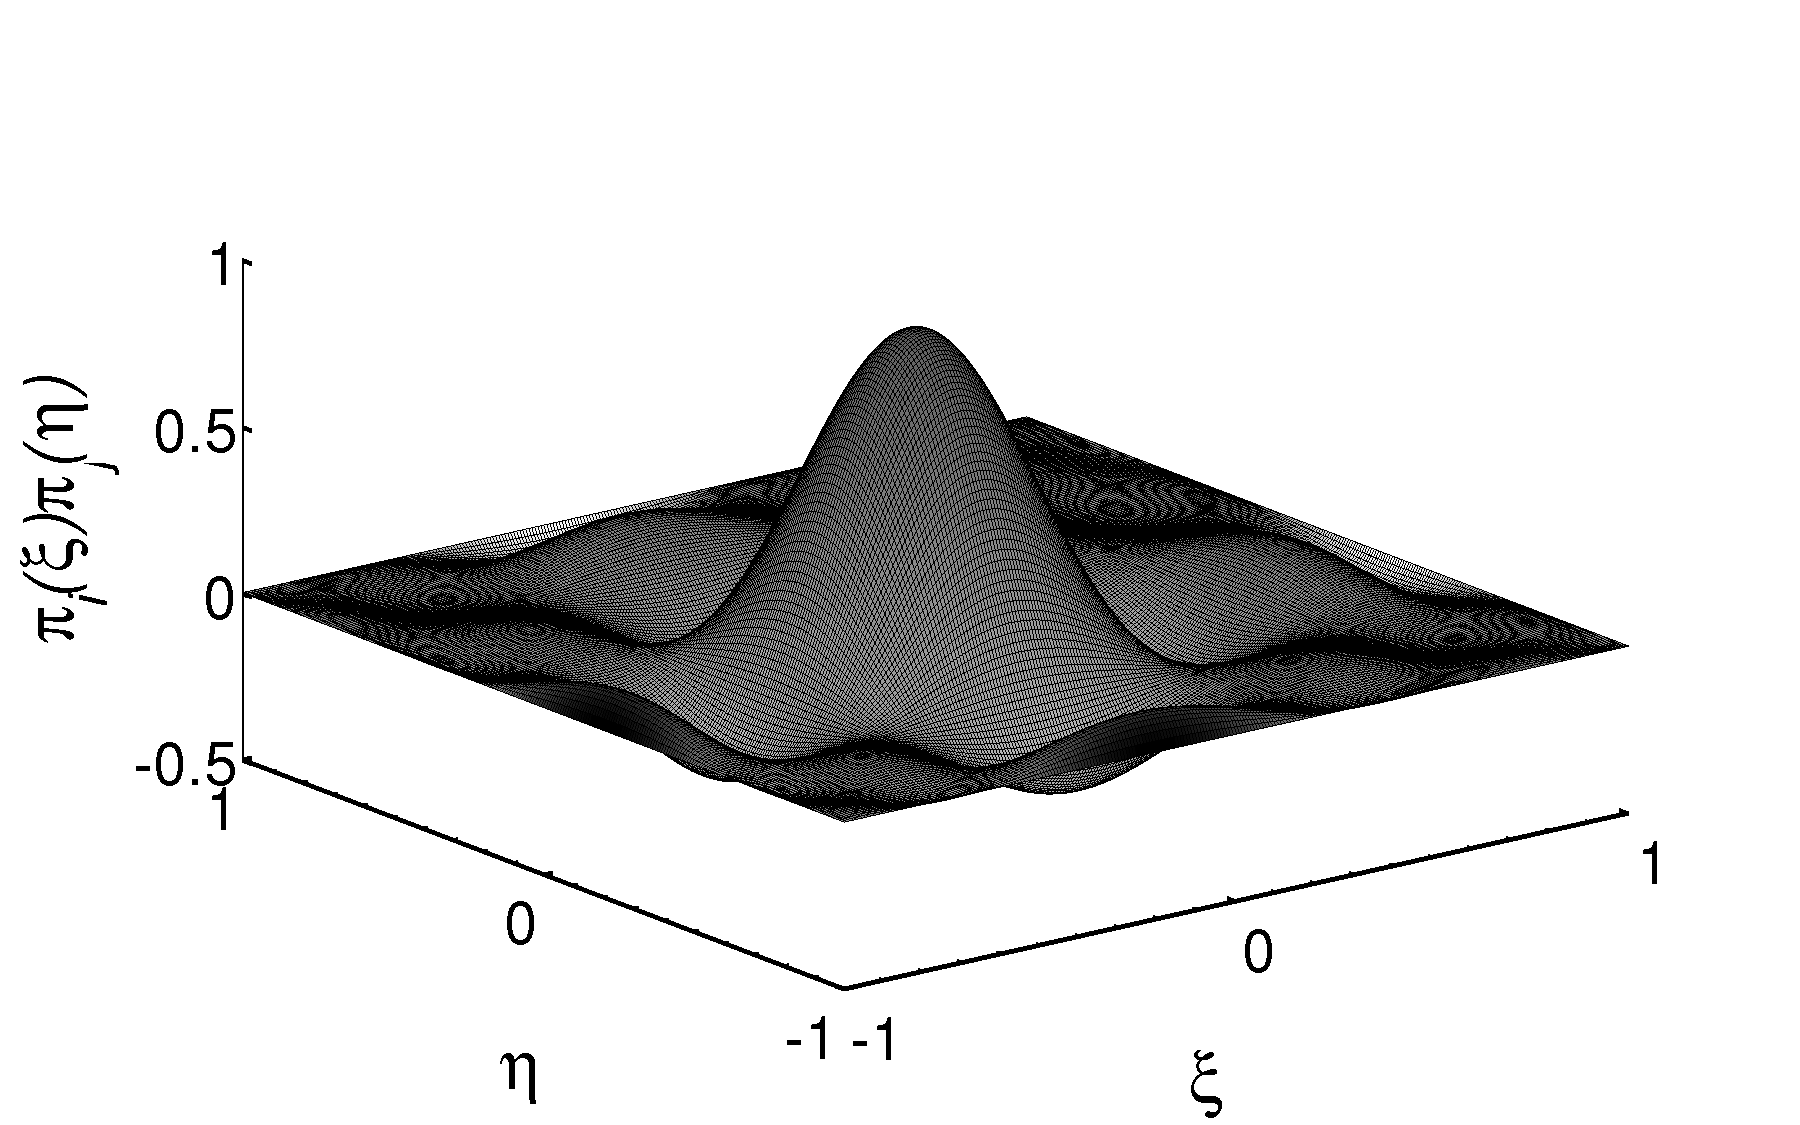
\includegraphics[width=\linewidth]{Figure/legpoly_2D2.pdf}
                 \caption{}
                 \label{fig:poly3}
         \end{subfigure}
        \caption[Lagrange-Legendre polynomial interpolants: $N = 7$]{(a) Lagrange-Legendre polynomial interpolant ${\pi_j}_{j=0}^{N}$ with $N = 7\,(\mbox{polynomial degree})$ in current SEM formulation. Blue $-+$,   $\pi_1(\xi)$;  Red $-\circ$,  $\pi_5(\xi)$;  Black $--\Box$,  $\pi_7(\xi)$; (b)$\  \pi_{1,1}(\xi,\eta) \ \ $ (c) $\  \pi_{4,4}(\xi,\eta) \ $. Figures (b), (c) obtained as Kronecker products of $\pi_{i}(\xi)\otimes \pi_{j}(\eta)$ for 2D case.}\label{fig:figure_legpoly1}
\end{figure}
The basis functions for expansion of the velocity variables correspond to Lagrange-Legendre interpolating polynomials,
\begin{equation}
\pi_{N,j}(\xi) = \prod_{i\neq j}\frac{\xi - \xi_j}{\xi_i - \xi_j} =  \frac{-1}{N(N+1)}\frac{(1-\xi^{2})L'_{N}(\xi)}{(\xi - \xi_j)L_N(\xi_j)}, \ \  \  \   0 \leq j \leq N, \  \  \ \  \xi \in [-1,1],  \label{legendre1}
\end{equation}
where $\xi_j$ are GLL quadrature nodes. Figure~\ref{fig:figure_legpoly1} shows the Lagrange-Legendre basis functions (Equation~(\ref{legendre1})) displaying the cardinality property, and they all have the common intersection point at the GLL quadrature nodes (roots of numerator of basis functions in Equation~(\ref{legendre1}) ) while $\pi_{j}(\xi) \ \mbox{and} \ \pi_{N-j}(\xi)$ basis functions have reflective symmetry about $\xi = 0$.

Likewise, it is legitimate to define the Lagrange interpolant basis functions for the pressure interpolants of degree $N-2$
\begin{equation}
\pi^{p}_{N,j}(\zeta) = \prod_{i\neq j}\frac{\zeta - \zeta_j}{\zeta_i - \zeta_j} = \frac{L_{N-1}(\zeta)}{(\zeta - \zeta_j)L'_{N-1}(\zeta_j)} , \ \  \  \   1 \leq j \leq N-1, \  \  \ \  \zeta \in [-1,1],  \label{legendre2}
\end{equation} 
\section{BDF$k$-EXT$k$ Scheme}\label{bdf}
The implicit Backward difference scheme of $k-th$ order (BDF$k$) using Taylor expansion of an ODE $u_t = g(u)$ can be given as
\begin{equation}
\frac{1}{\Delta t}\sum_{i=0}^{k}\beta_{i}u^{n+1-i} \approx g(u^{n+1})
\end{equation}
with $\Delta t$ being the time step and $\beta{i}$ are the BDF coefficients. To avoid the iterative form of non-linear non-symmetric system for implicit schemes of advection term, Karniadakis et. al~\cite{kar2} proposed a higher order extrapolation scheme on the non-linear terms (e.g. adevtion and other non-linear forcing). The $k'-th$ order extrapolation of a general non-linear term $g(u)$
\begin{equation}
g(u^{n+1}) \approx \sum_{i=1}^{k'}\alpha_{i}g(u^{n+1-i})
\end{equation}
with $\alpha_i$ being the extrapolation coefficients.
Combining the two schemes together generates BDF$k$/EXT$k$ scheme
\begin{equation}
\frac{1}{\Delta t}\sum_{i=0}^{k}\beta_{i}u^{n+1-i} \approx \sum_{i=1}^{k'}\alpha_{i}g(u^{n+1-i})
\end{equation}
with $k=k' \approx 2 \ \mbox{or} \ 3$
\begin{table}[ht] 
\centering % used for centering table 
\begin{tabular}{c c c c c c c} % centered columns (4 columns) 
\hline\hline    %inserts double horizontal lines 
$k$ & $\beta_0$ & $\beta_1$ & $\beta_2$ & $\beta_3$ & $\beta_4$ & $\beta_5$  \\ [0.5 ex] % inserts table 
%heading 
\hline  % inserts single horizontal line 
$1$ & $1$ & $-1$  \\
$2$ & ${3}/{2}$ & $-2$ & ${1}/{2}$  \\
$3$ & ${11}/{6}$ & $-3$ & ${3}/{2}$ & $-1/3$ \\
$4$ & ${25}/{12}$ & $-4$ & $3$ & $-{4}/{3}$ & $1/4$ \\
$5$ & ${137}/{60}$ & $-5$ & $5$ & $-{10}/{3}$ & $5/4$ & $-1/5$  \\
\hline \\ [1 ex]
\end{tabular} 
\caption[BDF Coefficients]{BDF coefficients $\beta_{i=0}^{k}$ for orders $k\ = \ 1-5$} % title of Table 
\label{table:BDF} % is used to refer this table in the text 
\end{table} 
\begin{table}[ht] 
\centering % used for centering table 
\begin{tabular}{c c c c} % centered columns (4 columns) 
\hline\hline    %inserts double horizontal lines 
$k$  & $\alpha_1$ & $\alpha_2$ & $\alpha_3$   \\ [0.5 ex] % inserts table 
%heading 
\hline  % inserts single horizontal line 
$1$ & $1$   \\
$2$ & ${2}$ & $-1$  \\
$3$ & $3$ & $-3$ & $1$ \\
\hline \\ [1 ex]
\end{tabular} 
\caption[EXT Coefficients]{EXT coefficients $\alpha_{i=1}^{k}$ for orders $k\ = \ 1-3$} % title of Table 
\label{table:EXT} % is used to refer this table in the text 
\end{table} 